In order to improve the energy consumption of this IoT system, it is possible modify multiple parameters:
\begin{itemize}
	\item transmission power for ESP-NOW communication;
	\item delay used to make a measurement with HC-SR04;
	\item time spent with WiFi turned on;
	\item time spent in deep sleep.
\end{itemize}

\section{Improvements for our implementation}
In our implementation, we use the lowest transmission power, of 2 dBm, and the lowest time, suggested by the documentation, of 10 $\mu \text{s}$ to make measurement with HC-SR04 ultrasonic sensor. Finally, we perform the board setup and the measurement with WiFi turned off.\\
Thus, the only parameter which we can modify to improve the system's lifetime is the deep sleep time. If we increased the time spent by the node in deep sleep, we would achieve a better lifetime, but we would need to tolerate a longer time to update the status of occupancy of the parking spot.\\
An alternative approach, consists in varying the frequency with which the node sends updates to the sink based on how the status of occupancy changes. If the status has changed over the last cycle, the node immediately notifies the sink; but, if the status doesn't change for a long time, the node can skip up to five transmission to the sink. If up to five transmissions are skipped, the sink can assume the occupancy value has not changed; after the fifth skipped transmission, the node notifies the sink with the occupancy value, which can be the same as the last one it sent, to inform it is still alive.\\
Thanks to this approach, when the status doesn't change, the node performs a measurement, computes the measured value and goes to deep sleep, instead of turning the WiFi on and transmitting data to the sink. Since the transmission represents a big part of the energy consumption of the node, we can increase the efficiency by a lot, without increasing the time needed to notify an update to the sink.\\

The power consumption of the ESP32 when the occupancy value doesn't changes is represented in the following plot.
\begin{figure}[H]
    \centering
    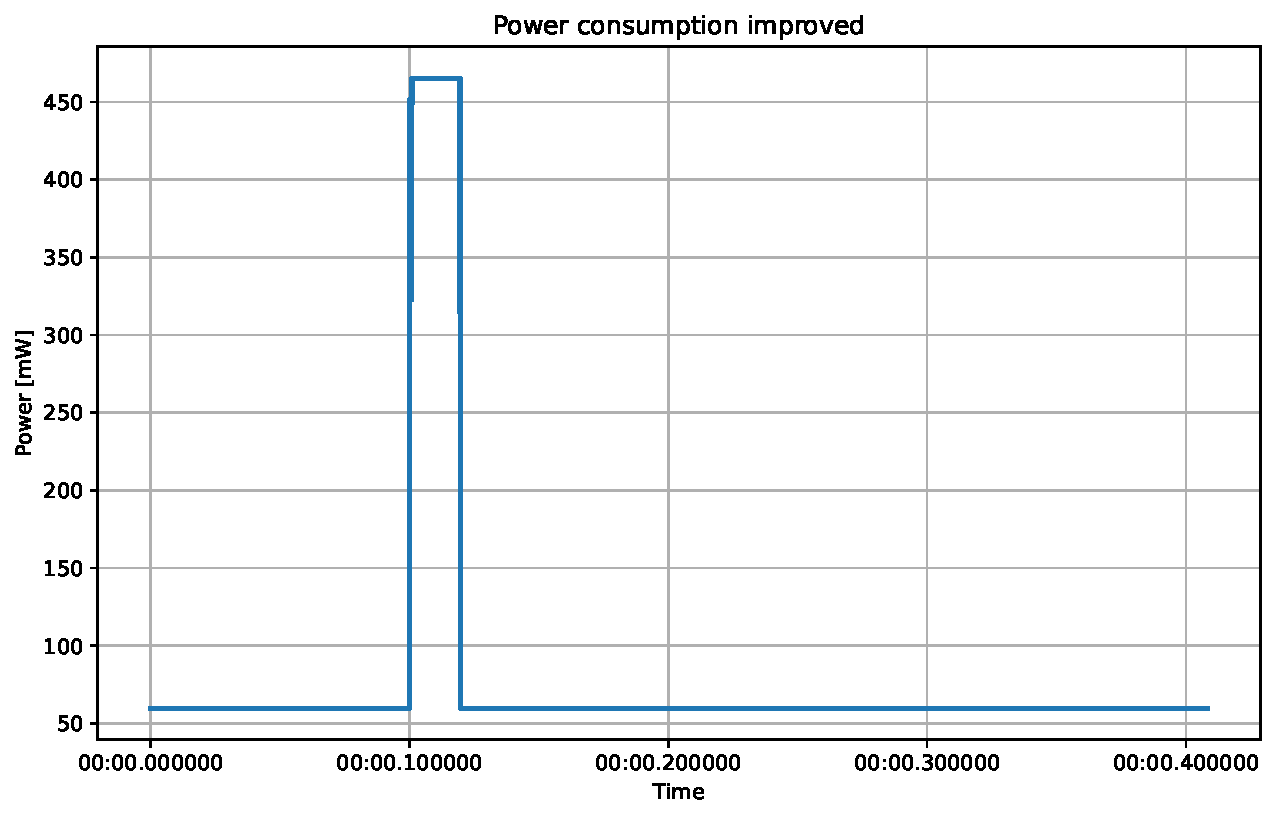
\includegraphics[width=\linewidth, height=0.4\textheight, keepaspectratio]{power_consumption_improved.pdf}
    \caption{Power consumption cycle without transmission}
    \label{fig:Power consumption cycle without transmission}
\end{figure}

We now compute the energy consumption of the node when the measurement doesn't change for 6 cycles, i.e. the ESP32 doesn't notify the sink for 5 times, since the measurement didn't change. This assumption looks reasonable, since this would mean that the occupancy of the parking spot, in the average situation, doesn't change more than one time every 5 minutes.\\
We compute the energy consumption for a cycle when the node doesn't notify the sink as:
\begin{align*}
E_{cycle}' = E_{idle} + E_{measurement} + E_{deep\_sleep}'
\end{align*}
Since we want to maintain a constant time for a cycle, the time spent in deep sleep is slightly higher, and can be computed as:
\begin{align*}
	T_{deep\_sleep}' = T_{cycle} - T_{idle} - T_{measurement} = 48.189 \text{s}\\
\end{align*}
The new energy consumption in deep sleep is:
\begin{align*}
	E_{deep\_sleep}' &= P_{deep\_sleep} \cdot T_{deep\_sleep}' = 2874.956\,\text{mJ} 
\end{align*}

Since the other values of energy consumptions are unchanged, we can compute the energy consumption of a cycle as:
\begin{align*}
	E_{cycle}' = E_{idle} + E_{measurement} + E_{deep\_sleep}' = 2883.899\,\text{mJ} 
\end{align*}
The energy consumption for 6 cycles, in which only one transmission is made is:
\begin{align*}
	E_{6\_cycles} = E_{cycle} + 5 \cdot E_{cycle}' = 17428.808\,\text{mJ} 
\end{align*}

The new sensor node's lifetime, measured in cycles, is:
\begin{align*}
	L_{cycles}&= 6 \cdot E_{b} / E_{6\_cycles} = 6400.782 \,\text{cycles} 
\end{align*}
The sensor will perform 6400 complete cycles and will die during the following one.

The total time for a cycle is always the same, $T_{cycle} = 48.208 s$, so the lifetime measured in time is of:
\begin{align*}
	L_{time}&= L_{cycles} \cdot T_{cycle} = 308568.899 \text{s}
\end{align*}

The new lifetime is equivalent to 3 days 13 hours 42 minutes and 48 seconds, which is more 3 hours longer than the base case.

\section{Improvements upper bound}
In order to put into perspective the energy efficiency of our system, we provide a theoretical upper bound of the system's lifetime, i.e. the lifetime when the deep sleep time tends toward infinity, the node always stays in deep sleep and isn't functional anymore.\\
The power consumption of the ESP32 in deep sleep mode is $P_{deep\_sleep} = 59.66\,\text{mW}$ and the battery life is $E_{b} = 18593\,\text{J}$, so the lifetime is:
\begin{align*}
	L_{time}&= E_{b} / P_{deep\_sleep} = 311649.346 \text{s}
\end{align*}

The lifetime of the system, when the deep sleep time tend towards infinity, is of 3 days 14 hours 34 minutes and 9 seconds, which is less than one our bigger than the improved version of the system.









